\section{Theorie}

\subsection{Furuata Pendel}
Bei dem Furuta Pendel handelt es sich um ein 1992 von Katsuhisa Furuta entwickeltes %nichtlineares Pendel
Modell. 

Test, ob Umlaute unterstützt werden: ÄÖÜß
Straße (Strasse)
Häuser (Haeuser)

\begin{figure}[htbp]
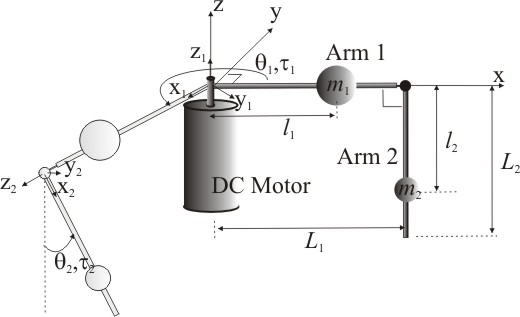
\includegraphics[width=0.8\textwidth]{Grafiken/furuta.jpg}
\caption{Furuta Pendel \colorbox{yellow}{Quelle: Wiki}}
\end{figure}


\begin{equation}
 E_{p1} = 0
\end{equation}

\begin{equation}
E_{k1}=\frac{1}{2}(v^T_{1c}m_1v_{1c}+\omega^T_1J_1\omega_1)=\frac{1}{2}\dot{\theta}^2_1(m_1l_1+J_{1zz})
\end{equation}

\begin{equation}
E_{p2}=gm_2l_2(\cos(\theta_2)-1)
\end{equation}

\begin{eqnarray}
E_{k2}&=&\frac{1}{2}(v^T_{2c}m_2v_{2c}+\omega^T_2J_2\omega_2)\nonumber \\
&=&\frac{1}{2}\dot{\theta}^2_1(m_2L^2_2+(m_2l^2_2+J_{2yy})\sin^2(\theta_2)+J_{2xx}\cos^2(\theta_2))\nonumber \\
&&+\frac{1}{2}\dot{\theta}^2_2(J_{2zz}+m_2l^2_2)+m_2L_1l_2\cos(\theta_2)\dot{\theta}_1\dot{\theta}_2
\end{eqnarray}

\begin{equation}
L=E_k-E_p
\end{equation}

\begin{equation}
\frac{d}{dt}(\frac{\partial L}{\partial\dot{q_i}})+b_i\dot{q}_i-\frac{\partial L}{\partial q_i}=Q_i
\end{equation}

\begin{equation}
\begin{bmatrix}
\tau_1 \\
\tau_2
\end{bmatrix}
=
\begin{bmatrix}
\begin{pmatrix}
\ddot{\theta}_1(J_{1zz}+m_1l^2_1+m_2L^2_1+(J_{2yy}+m_2l^2_2) 						\\
\times \sin^2(\theta_2)+J_{2xx}cos^2(\theta_2))+\ddot{\theta}_2m_2L_1l_2\cos(\theta_2)			\\
-m_2L_1l_2\sin(\theta_2)\dot{\theta}^2_2+\dot{\theta}_1\dot{\theta}_2\sin(2\theta_2)	\\
\times(m_2l^2_2+J_{2yy}-J_{2xx})+b_1\dot{\theta}_1
\end{pmatrix}
\\
\begin{pmatrix}
\ddot{\theta}_1m_2L_1l_2\cos(\theta_2)+\ddot{\theta}_2(m_2l^2_2+J_{2zz})	\\
+\frac{1}{2}\dot{\theta}_1\sin(2\theta_2)(-m_2l^2_2-J_{2yy}+J_{2xx})						\\
+b_2\dot{\theta}_2+gm_2l_2\sin(\theta_2)
\end{pmatrix}
\end{bmatrix}
\end{equation}

\begin{eqnarray}
J_1=
\begin{bmatrix}
J_{1xx} & 0 & 0\\
0 & J_{1yy} & 0\\
0 & 0 & J_{1zz}
\end{bmatrix}
\approx
\begin{bmatrix}
0 & 0 & 0\\
0 & J_{1} & 0\\
0 & 0 & J_{1}
\end{bmatrix}
\nonumber \\
J_2=
\begin{bmatrix}
J_{2xx} & 0 & 0\\
0 & J_{2yy} & 0\\
0 & 0 & J_{2zz}
\end{bmatrix}
\approx
\begin{bmatrix}
0 & 0 & 0\\
0 & J_{2} & 0\\
0 & 0 & J_{2}
\end{bmatrix}
\end{eqnarray}

\begin{eqnarray}
\hat{J}_1 &=& J_1 + m_1l^2_1	\nonumber	\\
\hat{J}_2 &=& J_2 + m_2l^2_2	\nonumber	\\
\hat{J}_0 &=& J_1 + m_1l^2_1 + m_2L^2_1
\end{eqnarray}

\begin{equation}
\begin{bmatrix}
\tau_1 \\
\tau_2
\end{bmatrix}
=
\begin{bmatrix}
\begin{pmatrix}
\ddot{\theta}_1(\hat{J}_0+\hat{J}_2\sin^2(\theta_2))+\ddot{\theta}_2m_2L_1l_2\cos(\theta_2)			\\
-m_2L_1l_2\sin(\theta_2)\dot{\theta}^2_2+\dot{\theta}_1\dot{\theta}_2\hat{J}_2\sin(2\theta_2)+b_1\dot{\theta}_1
\end{pmatrix}
\\
\begin{pmatrix}
\ddot{\theta}_1m_2L_1l_2\cos(\theta_2)+\ddot{\theta}_2\hat{J}_2-\frac{1}{2}\dot{\theta}^2_1\hat{J}_2\sin(2\theta_2)						\\
+b_2\dot{\theta}_2+gm_2l_2\sin(\theta_2)
\end{pmatrix}
\end{bmatrix}
\end{equation}


\colorbox{yellow}{Die folgenden Gleichungen enthalten noch den Fehler, den wir finden sollten.} \\
\colorbox{yellow}{Ich habe die Lösung gerade nicht parat.}
\begin{equation}
\ddot{\theta}_1 =
\frac{
\begin{bmatrix}
-\hat{J}_2b_1 \\ 
m_2L_1l_2\cos(\theta_2)b_2 \\ 
-\hat{J}^2_2\sin(2\theta_2) \\ 
-\frac{1}{2}\hat{J}_2m_2L_1l_2\cos(\theta_2)\sin(2\theta_2) \\ 
\hat{J}_2m_2L_1l_2\sin(\theta_2)
\end{bmatrix}^T
\begin{bmatrix}
\dot{\theta}_1 \\ 
\dot{\theta}_2 \\ 
\dot{\theta}_1\dot{\theta}_2 \\ 
\dot{\theta}^2_1 \\ 
\dot{\theta}^2_2
\end{bmatrix}
+
\begin{bmatrix}
\hat{J}_2 \\ 
-m_2L_1l_2\cos(\theta_2) \\ 
\frac{1}{2}m^2_2l^2_2L_1\sin(2\theta_2)
\end{bmatrix}^T
\begin{bmatrix}
\tau_1 \\ 
\tau_2 \\ 
g
\end{bmatrix} }
{\hat{J}_0\hat{J}_2+\hat{J}^2_2\sin^2(\theta_2)-m^2_2L^2_1l^2_2\cos^2(\theta_2)}
\end{equation}



\begin{equation}
\ddot{\theta}_2 =
\frac{
\begin{bmatrix}
m_2L_1l_2\cos(\theta_2)b_1 \\ 
-b_2(\hat{J}_0+\hat{J}_2\sin^2(\theta_2)) \\ 
m_2L_1l_2\hat{J}_2\cos(\theta_2)\sin(2\theta_2) \\ 
-\frac{1}{2}\sin(2\theta_2)(\hat{J}_0\hat{J}_2+\hat{J}^2_2\sin^2(\theta_2)) \\ 
-\frac{1}{2}m^2_2L^2_1l^2_2\sin(2\theta_2)
\end{bmatrix}
\begin{bmatrix}
\dot{\theta}_1 \\ 
\dot{\theta}_2 \\ 
\dot{\theta}_1\dot{\theta}_2 \\ 
\dot{\theta}^2_1 \\ 
\dot{\theta}^2_2
\end{bmatrix}
+
\begin{bmatrix}
-m_2l_2\cos(\theta_2) \\ 
\hat{J}_0+\hat{J}_2\sin^2(\theta_2) \\ 
-m_2l_2\sin(\theta_2)(\hat{J}_0+\hat{J}_2\sin^2(\theta_2))
\end{bmatrix}
\begin{bmatrix}
\tau_1 \\ 
\tau_2 \\ 
g
\end{bmatrix} }
{\hat{J}_0\hat{J}_2+\hat{J}^2_2\sin^2(\theta_2)-m^2_2L^2_1l^2_2\cos^2(\theta_2)}
\end{equation}

\begin{eqnarray}
\theta_{1e} &=& 0		\nonumber \\
\theta_{2e} &=& \pi	\nonumber \\
\dot{\theta}_{1e} &=& 0		\nonumber \\
\dot{\theta}_{2e} &=& 0	
\end{eqnarray}

\begin{equation}
\begin{bmatrix}
\dot{\theta}_1 \\ 
\dot{\theta}_2 \\ 
\ddot{\theta}_1 \\ 
\ddot{\theta}_2
\end{bmatrix}
=
\begin{bmatrix}
0 & 0 & 1 & 0 \\ 
0 & 0 & 0 & 1 \\ 
A_{31} & A_{32} & A_{33} & A_{34} \\ 
A_{41} & A_{42} & A_{43} & A_{44}
\end{bmatrix}
\begin{bmatrix}
\theta_1 \\ 
\theta_2 \\ 
\dot{\theta}_1 \\
\dot{\theta}_2
\end{bmatrix}
+
\begin{bmatrix}
0 & 0 \\ 
0 & 0 \\ 
B_{31} & B_{32} \\ 
B_{41} & B_{42}
\end{bmatrix}
\begin{bmatrix}
\tau_1 \\ 
\tau_2
\end{bmatrix}
\end{equation}

\begin{eqnarray}
A_{31} &=& 0	\nonumber \\
A_{32} &=& \frac{gm^2_2l^2_2L_1}{(\hat{J}_0\hat{J}_2-m^2_2L^2_1l^2_2)}	\nonumber \\
A_{33} &=& \frac{-b_1\hat{J}_2}{(\hat{J}_0\hat{J}_2-m^2_2L^2_1l^2_2)}	\nonumber \\
A_{34} &=& \frac{-b_2m_2l_2L_1}{(\hat{J}_0\hat{J}_2-m^2_2L^2_1l^2_2)}	\nonumber \\
A_{41} &=& 0	\nonumber \\
A_{42} &=& \frac{gm_2l_2\hat{J}_0}{(\hat{J}_0\hat{J}_2-m^2_2L^2_1l^2_2)}	\nonumber \\
A_{43} &=& \frac{-b_1m_2l_2L_1}{(\hat{J}_0\hat{J}_2-m^2_2L^2_1l^2_2)}	\nonumber \\
A_{44} &=& \frac{-b_2\hat{J}_0}{(\hat{J}_0\hat{J}_2-m^2_2L^2_1l^2_2)}	\nonumber \\
B_{31} &=& \frac{\hat{J}_2}{(\hat{J}_0\hat{J}_2-m^2_2L^2_1l^2_2)}	\nonumber \\
B_{41} &=& \frac{m_2L_1l_2}{(\hat{J}_0\hat{J}_2-m^2_2L^2_1l^2_2)}	\nonumber \\
B_{32} &=& \frac{m_2L_1l_2}{(\hat{J}_0\hat{J}_2-m^2_2L^2_1l^2_2)}	\nonumber \\
B_{42} &=& \frac{\hat{J}_0}{(\hat{J}_0\hat{J}_2-m^2_2L^2_1l^2_2)}	\nonumber \\
\end{eqnarray}

\begin{equation}
\tau=K_mi
\end{equation}
Herleitung der Parameter (1 zu 1 aus dem Dokument übernommen.. die Herangehensweise muss also noch verändert werden!):
\begin{eqnarray}
L_1 &=& l_a \nonumber \\
L_2 &=& l_{pm}
\end{eqnarray}
\begin{eqnarray}
m_1 &=& m_b+m_r+m_{sens} \nonumber \\
m_2 &=& m_p+m_{pm}
\end{eqnarray}

\begin{equation}
J_{arm} = m_r \frac{l^2_r}{12}+m_r(\frac{1}{2}l_r+l_b-l_a)^2
\end{equation}

\begin{equation}
J_{pend1}=m_bl^2_a
\end{equation}

\begin{equation}
J_{sens}=m_{sens}(l_a-l_b-l_r-\frac{1}{2}l_c)^2
\end{equation}

\begin{equation}
J_{ps}=m_p(r_b+\frac{1}{2}l_p)^2
\end{equation}

\begin{equation}
J_{pm}=m_{pm}l^2_{pm}
\end{equation}

\begin{equation}
J_{arm}+J_{pend1}+J_{sens}=m_1l^2_1J_{pm}+J_{ps}=m_2l^2_2
\end{equation}

\begin{equation}
l_1=\sqrt{\frac{m_r \frac{l^2_r}{12}+m_r(\frac{1}{2}l_r+l_b-l_a)^2+m_bl^2_a+m_{sens}(l_a-l_b-l_r-\frac{1}{2}l_c)^2}{m_1}}
\end{equation}

\begin{equation}
l_2=\sqrt{\frac{m_{pm}l^2_{pm}+m_p(r_b+\frac{1}{2}l_p)^2}{m_2}}
\end{equation}

... Hier sollten wir gucken, ob wie die Umformungen evtl. anders vornehmen.

\begin{eqnarray}
Liste der Zahlenwerte
\end{eqnarray}

\begin{equation}
\end{equation}

\begin{equation}
\end{equation}

Swing-Up
\begin{equation}
U = n \cdot g \cdot sign(E-E_0)\dot{\theta}_2\cos(\theta_2)
\end{equation}

\begin{equation}
E = E_{pot}+E_{kin}
\end{equation}

\begin{eqnarray}
E_{pot} &=& m_2gl_2(\cos(\theta_2)-1) \nonumber \\
E_{kin} &=& \frac{1}{2}\dot{\theta}^2_2\hat{J}_2
\end{eqnarray}

\begin{equation}
\end{equation}
